\documentclass[border=4pt,12pt]{standalone}
% House style for redrawn exam diagrams (diagram-v4: 0.4pt lines, filled -latex arrows, fine dashes; stipple and hatching drawn as real dots/lines (no PDF/SVG patterns, so they render in every browser and at any scale); transparent background). Every figure \input's this.
\usepackage{amsmath,amssymb}
\usepackage{txfonts}
\usepackage{pdfrender,xcolor}
% \halo{text}: label on shading. The shading stops just around each letter's outline (a thin knock-out that follows the
% glyphs, like the papers' typesetting), never a box. Owner: "I don't want a box around the text".
\newcommand{\halo}[1]{\leavevmode\rlap{\pdfrender{TextRenderingMode=2,LineWidth=2.2pt,LineJoinStyle=1,StrokeColor=white,FillColor=white}#1}#1}
\usepackage{tikz,pgfplots}
\pgfplotsset{compat=1.18}
\usetikzlibrary{arrows.meta,calc,angles,quotes,patterns,patterns.meta,intersections,positioning,decorations.markings,shapes.geometric}
% Stipple and hatching are drawn as actual dots / lines clipped to the region (path picture), NOT as pattern fills:
% SVG <pattern> fills vanish or blur when browsers scale the image, so the owner could not see the shading.
% Each dot is a 0.72pt square (keeps SVGs small; reads as a dot at print size). Dots sit on one global staggered grid, so neighbouring regions line up.
\makeatletter
\newdimen\ex@x \newdimen\ex@y \newdimen\ex@xa \newdimen\ex@ya \newdimen\ex@xb \newdimen\ex@yb \newcount\ex@row
\def\exam@stipplecolor{black!75}\def\exam@dotr{0.42pt}\def\exam@dotgap{2.5}
\def\ex@rowdots{\ifdim\ex@x<\ex@xb \pgfpathrectangle{\pgfqpoint{\dimexpr\ex@x-0.36pt\relax}{\dimexpr\ex@y-0.36pt\relax}}{\pgfqpoint{0.72pt}{0.72pt}}\advance\ex@x by \exam@dotgap pt\relax\expandafter\ex@rowdots\fi}
\def\exam@stipple{%
  \pgftransformreset% dots are sized in real points even inside scaled pictures
  \pgfpointanchor{path picture bounding box}{south west}\ex@xa=\pgf@x \ex@ya=\pgf@y
  \pgfpointanchor{path picture bounding box}{north east}\ex@xb=\pgf@x \ex@yb=\pgf@y
  \pgfsetfillcolor{\exam@stipplecolor}\pgfmathsetmacro\ex@h{\exam@dotgap/2}%
  \pgfmathtruncatemacro\ex@r{floor(\ex@ya/\ex@h)-1}\ex@row=\ex@r\relax
  \ex@y=\ex@r\dimexpr\ex@h pt\relax
  \loop\ifdim\ex@y<\ex@yb
    \pgfmathtruncatemacro\ex@c{floor(\ex@xa/\exam@dotgap)-1}\ex@x=\ex@c\dimexpr\exam@dotgap pt\relax
    \ifodd\ex@row \advance\ex@x by \ex@h pt\fi
    \ex@rowdots
    \advance\ex@y by \ex@h pt \advance\ex@row by 1
    \ifnum\numexpr\ex@row-(\ex@row/4)*4\relax=0 \pgfusepath{fill}\fi% flush every 4 rows: bounded TeX memory, few clip copies in the SVG
  \repeat\pgfusepath{fill}}
\newdimen\ex@d
\def\exam@hatch#1{% #1 = 1 for /, -1 for \ ; lines 45 degrees, 3pt apart
  \pgftransformreset
  \pgfpointanchor{path picture bounding box}{south west}\ex@xa=\pgf@x \ex@ya=\pgf@y
  \pgfpointanchor{path picture bounding box}{north east}\ex@xb=\pgf@x \ex@yb=\pgf@y
  \ex@d=\dimexpr\ex@yb-\ex@ya\relax \ex@x=\dimexpr\ex@xa-\ex@d\relax
  \loop\ifdim\ex@x<\ex@xb
    \ifnum#1>0 \pgfpathmoveto{\pgfqpoint{\ex@x}{\ex@ya}}\pgfpathlineto{\pgfqpoint{\dimexpr\ex@x+\ex@d\relax}{\ex@yb}}%
    \else \pgfpathmoveto{\pgfqpoint{\ex@x}{\ex@yb}}\pgfpathlineto{\pgfqpoint{\dimexpr\ex@x+\ex@d\relax}{\ex@ya}}\fi
    \advance\ex@x by 4.24pt
  \repeat
  \pgfsetlinewidth{0.4pt}\pgfsetstrokecolor{black}\pgfusepath{stroke}}
\def\examstipple{\exam@stipple}\def\examhatch{\exam@hatch}\def\examsetstipplecolor#1{\def\exam@stipplecolor{#1}}\def\examsetdotgap#1{\def\exam@dotgap{#1}}
\makeatother
% (legacy pattern kept for old files)
% staggered stipple like the NESA papers' dotted shading
\pgfdeclarepatternformonly{exam stipple}{\pgfpointorigin}{\pgfqpoint{2.2pt}{2.2pt}}{\pgfqpoint{2.2pt}{2.2pt}}{%
  \pgfpathcircle{\pgfqpoint{0.55pt}{0.55pt}}{0.42pt}\pgfpathcircle{\pgfqpoint{1.65pt}{1.65pt}}{0.42pt}\pgfusepath{fill}}
\tikzset{
  every picture/.style={line width=0.6pt, >={Latex[length=2mm,width=1.3mm]}},
  curve/.style={line width=0.6pt},
  open arrow/.style={-{Latex[length=2mm,width=1.3mm]}},  % owner: filled -latex heads everywhere, no open chevrons
  aux/.style={dash pattern=on 2pt off 1.5pt, line width=0.6pt},
  shade/.code={\def\exA{#1}\def\exB{none}\ifx\exA\exB\else\pgfkeysalso{fill=black!18}\fi},
  shade/.default=on,
  shade dots/.style={fill=none, path picture={\examstipple}},
  stipple color/.code={\examsetstipplecolor{#1}},
  stipple gap/.code={\examsetdotgap{#1}},
  shade dense dots/.style={fill=none, stipple gap=1.6, path picture={\examstipple}},
  shade hatch/.style={fill=none, path picture={\examhatch{1}}},
  shade hatch reverse/.style={fill=none, path picture={\examhatch{-1}}},
  shade solid/.style={fill=black},
  pt/.style={circle, fill, inner sep=1.1pt},
  open pt/.style={circle, draw, fill=white, inner sep=1.1pt},
}
\pgfplotsset{
  exam axes/.style={axis lines=middle, axis line style={->}, xlabel={$x$}, ylabel={$y$},
    xlabel style={anchor=west}, ylabel style={anchor=south}, tick label style={font=\small},
    every axis plot/.append style={line width=0.6pt, black}, samples=200, clip=false,
    enlargelimits=false, axis on top},
}

\begin{document}
% graph of y=f(x); 1 unit = 49.8 px
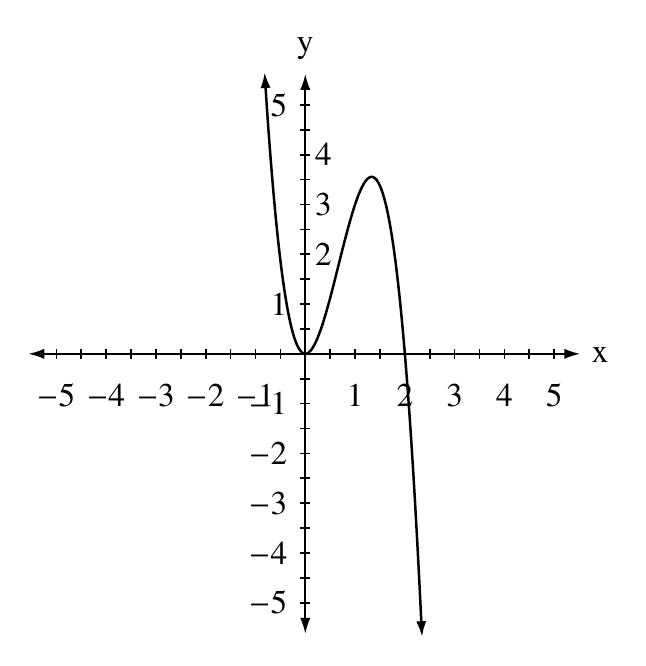
\begin{tikzpicture}[x=0.0127cm,y=-0.0127cm,every node/.style={font=\fontsize{12}{14}\selectfont}]
  \draw[<->] (25.1,338.0) -- (576.9,338.0);
  \draw[<->] (302.0,617.9) -- (302.0,58.1);
  \draw (53.0,333.0) -- (53.0,343.0); \draw (297.0,587.0) -- (307.0,587.0);
  \draw (77.9,333.0) -- (77.9,343.0); \draw (297.0,562.1) -- (307.0,562.1);
  \draw (102.8,333.0) -- (102.8,343.0); \draw (297.0,537.2) -- (307.0,537.2);
  \draw (127.7,333.0) -- (127.7,343.0); \draw (297.0,512.3) -- (307.0,512.3);
  \draw (152.6,333.0) -- (152.6,343.0); \draw (297.0,487.4) -- (307.0,487.4);
  \draw (177.5,333.0) -- (177.5,343.0); \draw (297.0,462.5) -- (307.0,462.5);
  \draw (202.4,333.0) -- (202.4,343.0); \draw (297.0,437.6) -- (307.0,437.6);
  \draw (227.3,333.0) -- (227.3,343.0); \draw (297.0,412.7) -- (307.0,412.7);
  \draw (252.2,333.0) -- (252.2,343.0); \draw (297.0,387.8) -- (307.0,387.8);
  \draw (277.1,333.0) -- (277.1,343.0); \draw (297.0,362.9) -- (307.0,362.9);
  \draw (326.9,333.0) -- (326.9,343.0); \draw (297.0,313.1) -- (307.0,313.1);
  \draw (351.8,333.0) -- (351.8,343.0); \draw (297.0,288.2) -- (307.0,288.2);
  \draw (376.7,333.0) -- (376.7,343.0); \draw (297.0,263.3) -- (307.0,263.3);
  \draw (401.6,333.0) -- (401.6,343.0); \draw (297.0,238.4) -- (307.0,238.4);
  \draw (426.5,333.0) -- (426.5,343.0); \draw (297.0,213.5) -- (307.0,213.5);
  \draw (451.4,333.0) -- (451.4,343.0); \draw (297.0,188.6) -- (307.0,188.6);
  \draw (476.3,333.0) -- (476.3,343.0); \draw (297.0,163.7) -- (307.0,163.7);
  \draw (501.2,333.0) -- (501.2,343.0); \draw (297.0,138.8) -- (307.0,138.8);
  \draw (526.1,333.0) -- (526.1,343.0); \draw (297.0,113.9) -- (307.0,113.9);
  \draw (551.0,333.0) -- (551.0,343.0); \draw (297.0,89.0) -- (307.0,89.0);
  \node at (53.0,380.0) {$-5$};
  \node[anchor=east] at (294.0,587.0) {$-5$};
  \node at (102.8,380.0) {$-4$};
  \node[anchor=east] at (294.0,537.2) {$-4$};
  \node at (152.6,380.0) {$-3$};
  \node[anchor=east] at (294.0,487.4) {$-3$};
  \node at (202.4,380.0) {$-2$};
  \node[anchor=east] at (294.0,437.6) {$-2$};
  \node at (252.2,380.0) {$-1$};
  \node[anchor=east] at (294.0,387.8) {$-1$};
  \node at (351.8,380.0) {$1$};
  \node[anchor=east] at (294.0,288.2) {$1$};
  \node at (401.6,380.0) {$2$};
  \node[anchor=west,inner sep=0pt] at (311.0,238.4) {$2$};
  \node at (451.4,380.0) {$3$};
  \node[anchor=west,inner sep=0pt] at (311.0,188.6) {$3$};
  \node at (501.2,380.0) {$4$};
  \node[anchor=west,inner sep=0pt] at (311.0,138.8) {$4$};
  \node at (551.0,380.0) {$5$};
  \node[anchor=east] at (294.0,89.0) {$5$};
  \node at (596.9,339.0) {x};
  \node at (302.0,32.1) {y};
  \draw[<->, line width=0.9pt] plot[domain=-0.818:2.345,smooth,samples=90] ({302.00+49.800*(\x)},{338.00-49.800*(6*(\x)^2-3*(\x)^3)});
\end{tikzpicture}
\end{document}
